\documentclass{article}[IEEEtran]
\usepackage[a4paper,
            left=1in,right=1in,top=1in,bottom=0.5in,
            footskip=.25in]{geometry}
\usepackage[utf8]{inputenc}
\usepackage{siunitx} % Provides the \SI{}{} and \si{} command for typesetting SI units
\usepackage{graphicx} % Required for the inclusion of images
\usepackage{amsmath} % Required for some math elements 
\usepackage{caption}
\usepackage{tikz}
\usepackage{import}
\usepackage{fancyhdr}
\usepackage[english]{babel}
\usepackage{algorithm}
\usepackage[noend]{algpseudocode}
\usepackage{pdfpages}
\usepackage{setspace}
\setlength\parindent{0pt} % Removes all indentation from paragraphs
\usepackage[export]{adjustbox}
\newcommand{\HRule}{\rule{\linewidth}{0.5mm}}
\usepackage{wrapfig}
\usepackage[font=scriptsize]{caption}
\usepackage{minted}
\usepackage{booktabs}
\usepackage{graphicx}
\usepackage{listings}
\definecolor{delim}{RGB}{20,105,176}
\definecolor{numb}{RGB}{106, 109, 32}
\definecolor{string}{rgb}{0.64,0.08,0.08}
\usepackage{setspace}

\lstdefinelanguage{json}{
    numbers=left,
    numberstyle=\small,
    frame=single,
    rulecolor=\color{black},
    showspaces=false,
    showtabs=false,
    breaklines=true,
    postbreak=\raisebox{0ex}[0ex][0ex]{\ensuremath{\color{gray}\hookrightarrow\space}},
    breakatwhitespace=true,
    basicstyle=\ttfamily\small,
    upquote=true,
    morestring=[b]",
    stringstyle=\color{string},
    literate=
     *{0}{{{\color{numb}0}}}{1}
      {1}{{{\color{numb}1}}}{1}
      {2}{{{\color{numb}2}}}{1}
      {3}{{{\color{numb}3}}}{1}
      {4}{{{\color{numb}4}}}{1}
      {5}{{{\color{numb}5}}}{1}
      {6}{{{\color{numb}6}}}{1}
      {7}{{{\color{numb}7}}}{1}
      {8}{{{\color{numb}8}}}{1}
      {9}{{{\color{numb}9}}}{1}
      {\{}{{{\color{delim}{\{}}}}{1}
      {\}}{{{\color{delim}{\}}}}}{1}
      {[}{{{\color{delim}{[}}}}{1}
      {]}{{{\color{delim}{]}}}}{1},
}


\lstset{language=json} 

\renewcommand{\labelenumi}{\alph{enumi}.} % Make numbering in the enumerate environment by letter rather than number (e.g. section 6)

%\usepackage{times} % Uncomment to use the Times New Roman font

            
\pagestyle{fancy}
\pagenumbering{arabic}
\fancyhf{}
\fancyfoot[C]{\thepage}
\fancyhead[L]{\nouppercase SMBUD Project - MongoDB}


\begin{document}
%===========================================================
\begin{titlepage}
\begin{center}

\captionsetup{font=footnotesize}

% Top 
\textsc{AY 2021-2022}\\[2cm]


\includegraphics[width=0.55\textwidth]{logo.png}~\\[2cm]


% Title
\HRule \\[0.4cm]
{ \LARGE 
  \textbf{SMBUD Project}\\[0.4cm]
  \emph{Covid Certificates-Oriented MongoDB Database}\\[0.4cm]
}
\HRule \\[1.5cm]



% Author
\begin{center}
    {\large Pablo Giaccaglia - 10626428\\[0.1cm]  Santi Pier Pistone - 10867402 \\[0.1cm]    Salvatore Cassata - 10560790\\[0.1cm]  Stefano Vighini - 10622788\\[0.1cm]  Zhitao He - 10763530\\[0.1cm] 
}
\end{center}

\vfill

\textsc{\large Master of Science in \\Computer Science \& Engineering}\\[0.4cm]


% Bottom
{\large \today}
 
\end{center}
\end{titlepage}

\newpage


%===========================================================
\tableofcontents
\addtocontents{toc}{\protect\thispagestyle{empty}}
\newpage
\setcounter{page}{1}

%===========================================================
%===========================================================
\section{Introduction}\label{sec:intro}

This project's purpose is to keep track of \textbf{COVID-19 pandemic} data about people, authorized bodies, vaccines, tests and, most of all, Covid certificates of vaccination or testing by designing and implementing a document-based \textbf{MongoDB} database. The primary objective is to support a fast tool that checks the validity of the certificate. 
The data stored allows to extract actionable insights concerning various statistical purposes, involving information such as health services, vaccination \& testing hubs and vaccine lots, even though the database is not optimized for these tasks, since the already mentioned main goal regards certificates validity check.

\section{Specification \& Hypothesis}\label{sec:spec-hyp}

In order to fulfill the purpose described in the introduction, we created a database with just 3 type of MongoDB documents, managed within their homonym collections:
\begin{itemize}
\item \textbf{people}, that include all available and necessary demographic information and about people's certification of vaccines and tests.
\item \textbf{healthcare services}, with main information and also its hubs (where the vaccine or the test has been taken)
\item \textbf{vaccine lots}. This entity containins specific information about the vaccine lot.
\end{itemize}
We chose to put the core information in the main document '\textbf{Person}', and additional information in other documents. These can be retrieved with an aggregation, but the idea is that these shouldn't be the main accessed data for every-day use.

\section{Data Model}\label{sec:data}

\subsection{ER Diagram}

\begin{figure}[H]
\begin{center}
    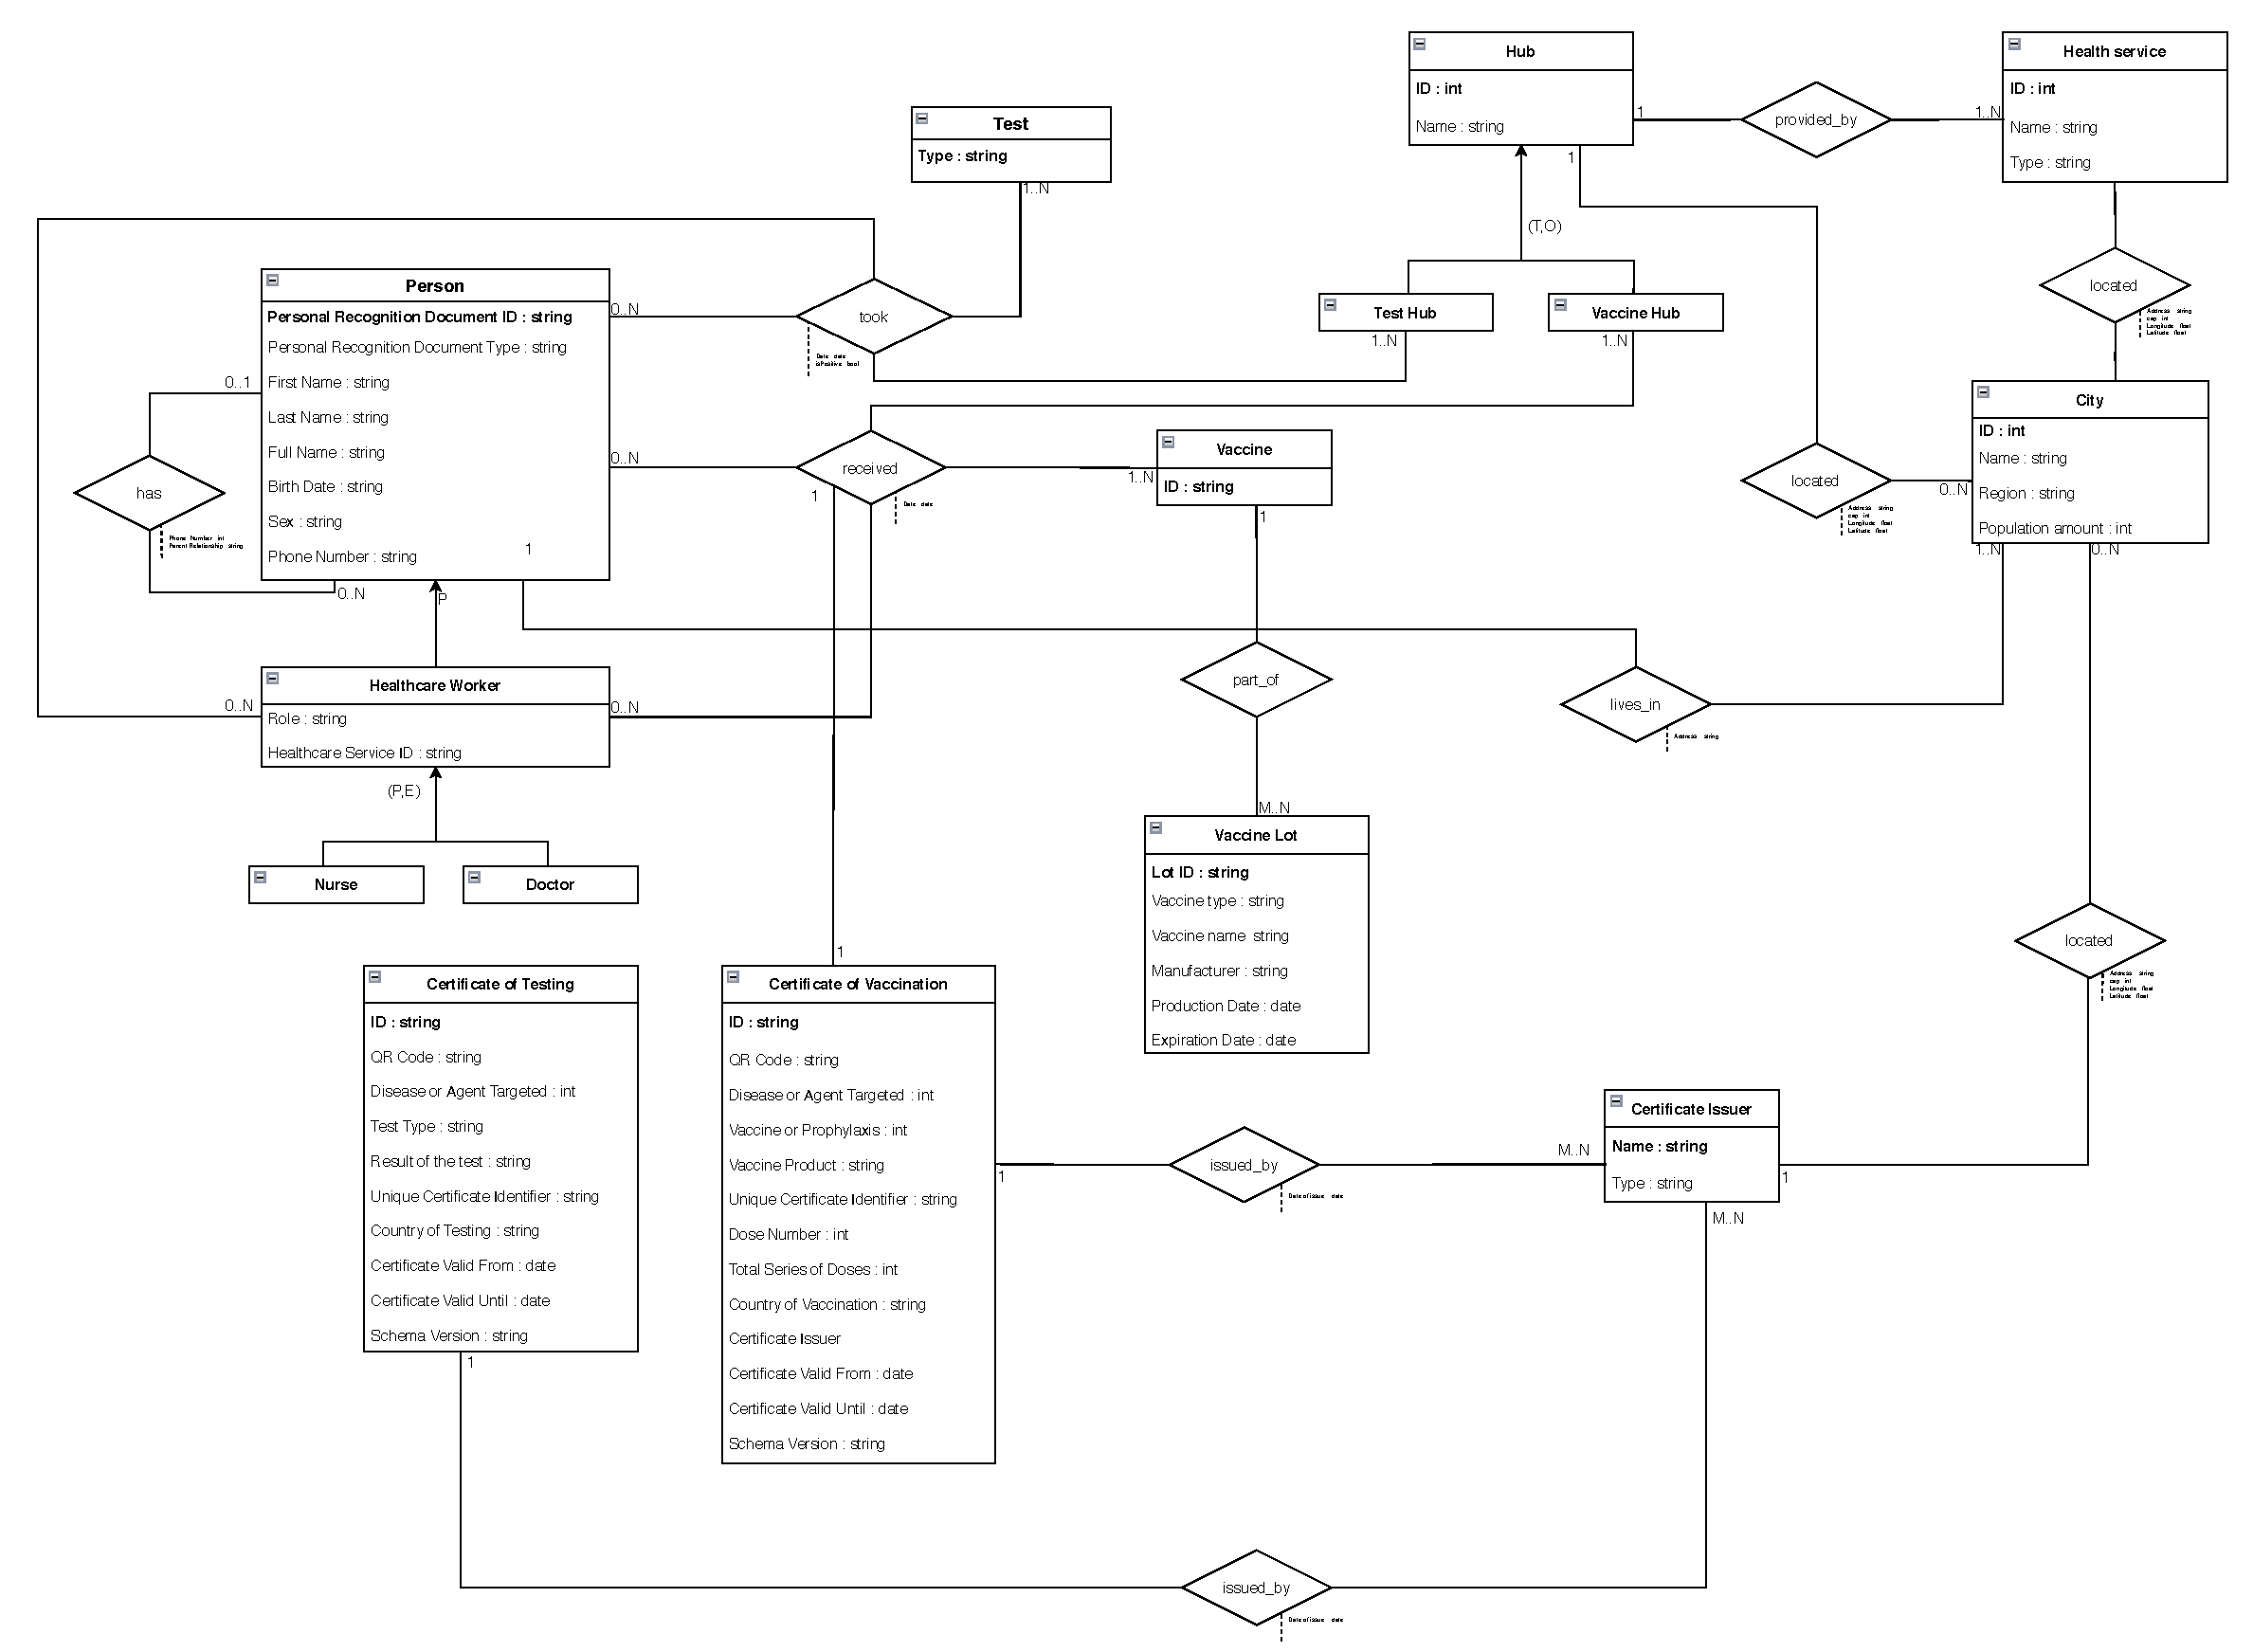
\includegraphics[width=\textwidth]{mongdb-er.pdf}
    \caption{ER Diagram}
\end{center}
\end{figure}

\subsection{Document Diagram}

\begin{figure}[H]
\begin{center}
    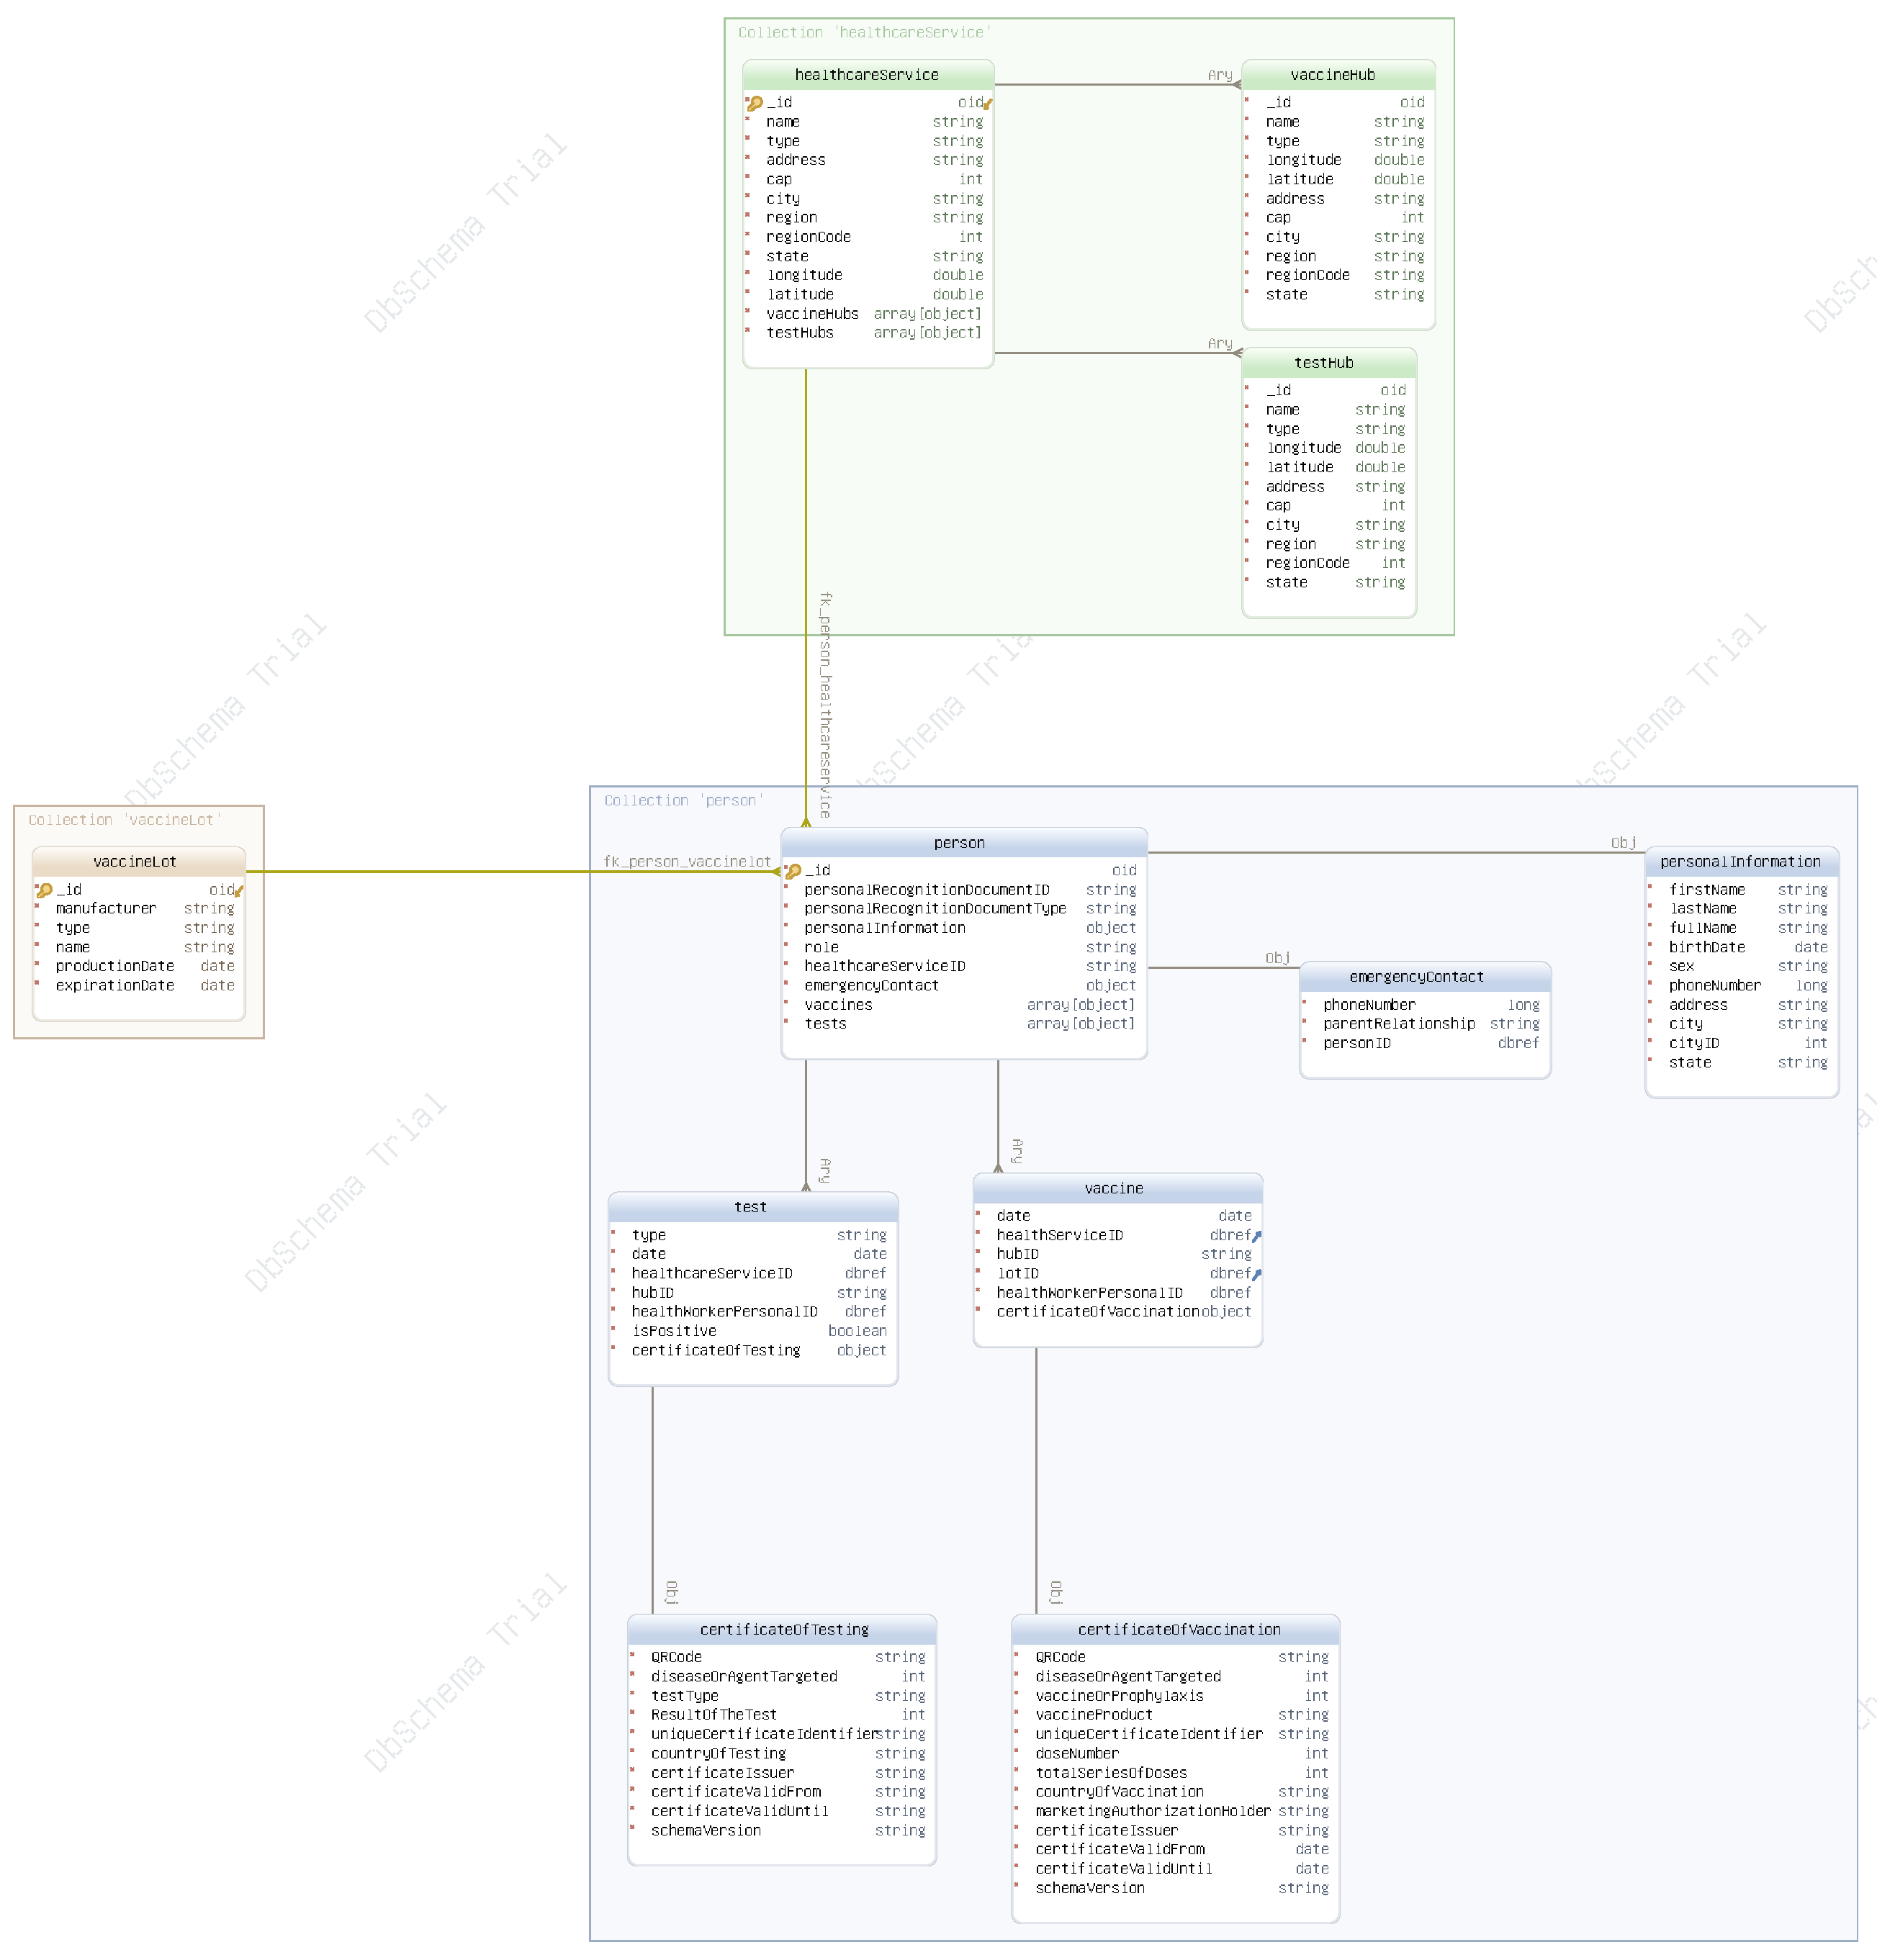
\includegraphics[width=\textwidth]{mongodb-docdiagram.pdf}
    \caption{Document Diagram}
\end{center}
\end{figure}


\subsection{From ER to document}

The translation of the ER schema in a document approach was not straight forward. We chose to keep some entities, we pushed others inside the 'main' entity. We chose the main entity to be 'person', as our main goal is to verify people's certificates and this entity should be the 'key' of our searches. 
\\
Then, there are 2 additional root documents, \textbf{HealthcareService} and \textbf{VaccineLot}, as they are not related to the person itself. This decision made the database lighter and a bit more readable. Further details will be provided. 
\\\\
Our key reasoning was based on: 

\begin{itemize}
    \item simplify the entities that are not strictly important ('cities') and push their content in related entities
    \item choose one main entity per group and 'walk through' the relationships to create sub-documents.
\end{itemize} 

To achieve these goals ad-hoc alterations were needed.
\newpage
One example of modification is that we decided to merge in some ways the vaccine and certificate, but keeping the difference (that will be explained in the next subsection '\textbf{Design choices}').
\\
Another decision we made is that when one sub-entity is shared between 2 main entities (for example, the hub, \textbf{VaccineHub} or \textbf{TestHub}, shared between \textbf{HealthcareService} document and \textbf{Test}/\textbf{Vaccine} document), it will be stored as a sub-document in the more entailed one, and as a reference in the other one.
\\
We also grouped some information in sub-documents that didn't exist in the ER, like '\textbf{personalInformation}', just for readability purposes.


\subsection{Design choices}

\begin{itemize}
\item \textbf{information about vaccine lots}. We chose to separate this information from the vaccine in the person just because this data is not so important for our purposes. So, as it may be very redundant, and not so queried, we've put it in a different entity.
\item \textbf{people that are nurses or doctors}. As stated in the ER diagram, a person can be either a nurse, a doctor or none of them. To distinguish, we kept the same schema for all people, including the role and the healthcareServiceID. If the person is a 'normal' one, these fields are set to null.
\item \textbf{city information.} Not to overload the database with a lot of entities, we chose to push all information about cities in the respective documents and sub-documents.
\item \textbf{vaccines, tests and certificates}. We chose to put at the first level of '\textbf{vaccines}' and '\textbf{tests}' array (in the '\textbf{person}' document) the information related and useful for our database. To stick to reality, we also put inside of it a sub-document '\textbf{certificate}' that emulates the Green Pass (only in part). Therefore this data is also pretty difficult to query, as it is 'encoded' and structured by a third-party entity (the certificate issuer). 
\end{itemize}


\section{Database Creation}\label{sec:creation}

The database creation process has relied on various \textbf{CSV} datasets freely available online and on \textbf{Python}\cite{van1995python} programming language, in order to extract the information suitable to build an appropriate dataset \\ fulfilling our needs. Since information comes from different providers, such as public companies \\ (e.g \textbf{DatiOpen.it, dati.salute.gov.it, ec.europa.eu/health}), the need to have a data processing pipeline was high.
Thus through several Python functions and libraries we sequentially applied different modification to data, including:

\begin{itemize}
    \item Null fields rows removal
    \item Duplicate rows removal
    \item Standardization of fields to have only first letter uppercase
    \item Document delimiter conversion to match CSV standard (e.g from "\textbf{;}" to "\textbf{,}" delimiter)
    \item Generation of random documents IDs, with respect to the real document number format \\ (e.g : 2 letters and 7 digits for Italian passport number)
    \item  Geographical information (e.g geographic coordinates, address) of places with \textbf{GMaps Geocoding API}\cite{GMapsAPI} by providing partial information (e.g : name and the region of a pharmacy), since most of the datasets found online often have incomplete information.
    \item Generation of random birth dates, phone numbers and assignment of random emergency contacts (including phone number, parental relationship and person ID), residence address, Covid tests, vaccine doses and their respective hubs of administration to people.
\end{itemize}

The MongoDB philosophy according to which a collection does not require its documents to have the same schema was partially adopted, since instead of having missing fields the document stores null values. This choice was made to ease the bulk population of the database through the Python PyMongo Driver, anyway the database can be adapted to a schema-less or a document validation enforcement structure.
\\ 
In the following sections, for each collection of the database we provide a brief description of particular problems we had to face during the data retrieval process. 

\subsection{Collection 'person'}

This collection contains the core documents of the database, storing all the information related to a person concerning Covid certificates.
The 'person' document is composed by several fields, including embedded documents and references to other documents.

Non Object or Array fields are:

\begin{itemize}
    \item \textbf{\_id}: objectId of mongoDB. It corresponds to the encoding of 'personalRecognitionDocumentID'
    \item \textbf{personalRecognitionDocumentID}: the documentID used to identify the person in real life.
    \item \textbf{personalRecognitionDocumentType}: the type of the above document, which is, in the current database storing italian data, one of the following:
    \begin{itemize}
        \item Italian passport
        \item Italian electronic identity card
        \item Italian driving license card
    \end{itemize}
    \item \textbf{role}: 'nurse', 'doctor' or null.
    \item \textbf{healthcareServiceID}: the documentID, if the person is a nurse or doctor, null if not.
\end{itemize}

The array fields are:

\begin{itemize}
    \item \textbf{vaccines}: list of received vaccines.
    \item \textbf{test}: list of taken tests.
\end{itemize}

Finally among the document's field there are several objects and subobjects, which are analyzed in the following subsections.

\subsubsection{SubDocument 'personalInformation'}

This document contains demographic details of a person, such as the first name and the phone number.

The original data comes from the \textbf{2019 Facebook breach}\cite{facebookleak}. We selected a single text file coming from the Italian section of the dump, firstly reduced the amount of information (original file size is around \textbf{800 MB}) to 5000 entries, then we parsed it, dealing with a non standard data record format, removed unused information (such as relationship status) and added random realistic information (such as birth date).

In particular the document's fields are:

\begin{itemize}
    \item \textbf{firstName}
    \item \textbf{lastName}
    \item \textbf{fullName}
    \item \textbf{birthDate}
    \item \textbf{sex}
    \item \textbf{phoneNumber} 
    \item \textbf{address}
    \item \textbf{city}
    \item \textbf{state}
\end{itemize}

\subsubsection{SubDocument 'emergencyContact'}

This document contains minimum information about an emergency contact person. The document is composed by the following fields:

\begin{itemize}

    \item \textbf{phoneNumber}
    \item \textbf{parentalRelationship}: degree of kinship with the main person. if the subdocument is not null, the value of this fields in the current database is one of the following: 
    \begin{itemize}
        \item spouse
        \item sibling
        \item friend
        \item father
        \item mother
        \item son
        \item daughter
        \item nephew
        \item friend
    \end{itemize}
    
    \item \textbf{personID}: DBRef to the person. It has to be underline that this is not really an ID, but an object containing \$ref, \$id, and \$db fields according to which is the correct way to handle \textbf{MongoDB references}\cite{mongodbreferences}.
    
\end{itemize}

\newpage
\subsubsection{SubDocument 'vaccine'}
Element of the '\textbf{vaccines}' array.

This document contains all the information regarding a vaccine dose, organized into 2 "groups".
The first group is composed by several fields storing information about administration place, date and healthcare personnel. 
In particular these fields are:

\begin{itemize}
    \item \textbf{date} : Date of the vaccination. In the database this value ranges from \textbf{2021-01-05} to \textbf{2021-05-30}
    
    \item \textbf{healthServiceID}: randomly generated 24 digits hexadecimal code identifying a health service organization operating in a certain area. In the database these ids are related to italian '\textbf{ASL}' Offices. It has to be underlined that this is not really an ID, but an object containing \$ref, \$id, and \$db fields according to which is the correct way to handle \textbf{MongoDB references}\cite{mongodbreferences}.
    
    \item \textbf{hubID}: randomly generated 24 digits hexadecimal code identifying a vaccination hub.
    
    \item \textbf{lotID}: randomly generated 24 digits hexadecimal code identifying a vaccine lot. It has to be underlined that this is not really an ID, but an object containing \$ref, \$id, and \$db fields according to which is the correct way to handle \textbf{MongoDB references}\cite{mongodbreferences}.
    
    \item \textbf{healthWorkerPersonID}: randomly generated 24 digits hexadecimal code representing the fixed length hex encoding of the personalRecognitionDocumentID belonging to the healthcare worker who administered the dose. It has to be underlined that this is not really an ID, but an object containing \$ref, \$id, and \$db fields according to which is the correct way to handle \textbf{MongoDB references}\cite{mongodbreferences}.
    
\end{itemize}

The second group composed by a '\textbf{certificateOfVaccination}' Object, which is analyzed in the following subsection.

\subsubsection{SubSubDocument 'certificateOfVaccination'}

This document contains information which reflects a real green certificate. In fact its fields (excepting the \textbf{QRCode} field) are compliant to the official \textbf{European eHealth network COVID certificate JSON Schema Specification}\cite{euDigitalCovid}, even though not all the specified fields are here included. In particular these fields are :

    \begin{itemize}
        \item \textbf{QRCode}: This string value represent the encoded JSON '\textbf{certificateOfVaccination}' document, excluding this field. The process for producing this remotely mimics what the \textbf{European eHealth Trust Framework for Certificates}\cite{euSecurity} expects. The process we applied is the following:
        
        \begin{itemize}
            \item JSON Dump of the Python dictionary representing the certificate.
            \item UTF-8 encoding of the JSON string.
            \item Base 45 encoding of the bytes generated by the previous encoding.
            \item Compression with zlib of the previously generated bytes.
            \item QR Code Image generation with qrcode Python library.
            \item Base 64 encoding of image bytes.
            \item Bytes conversion to string.
        \end{itemize}
        
        Through appropriate functions the process can be performed backwards to obtain both the QR Code and the original JSON string.
        
        \item \textbf{diseaseOrAgentTargeted}: This value set has a single entry \textbf{840539006} , which is the code for COVID19 from 
        SNOMED CT.
        \item \textbf{vaccineOrProphylaxis}: \textbf{SNOMED CT} code indicating the vaccine or prophylaxis used. The mapping is the following: 
        \begin{itemize}
            \item \textbf{SARS-CoV2 antigen vaccine}: 1119305005
            \item \textbf{SARS-CoV2 mRNA vaccine}: 1119349007
        \end{itemize}
        
        \item \textbf{vaccineProduct}: Code complying the Union Register of medicinal products code system representing Medicinal product used for the specific dose of vaccination, The mapping is the following:
        
        \begin{itemize}
            \item \textbf{Pfizer Vaccine}: EU/1/20/1528
            \item \textbf{Moderna Vaccine}: EU/1/20/1507
            \item \textbf{AstraZeneca Vaccine}: EU/1/21/1529
            \item \textbf{Janssen Vaccine}: EU/1/20/1525 
        \end{itemize}
        
        \item \textbf{uniqueCertificateIdentifier}: Unique certificate identifier (\textbf{UVCI}), whose structure mimics the one specified in this document only in terms of sequence of digits and characters.
        
        \item \textbf{doseNumber}:Sequence number (positive integer) of the dose given during a vaccination event. 1 for the first dose, 2 for the second dose etc.
        
        \item \textbf{totalSeriesOfDoses}: Total number of doses (positive integer) in a complete vaccination series according to the used vaccination protocol. In the database this value is set to 1 for "Janssen" vaccine certificate, 2 in all the other cases.
        
        \item \textbf{countryOfVaccination}: Country expressed as a 2-letter ISO3166 code. In the current database this value is 'IT', since the data regards Italy.
        
        \item \textbf{marketingAuthorizationHolder}: Marketing authorisation holder code from \textbf{EMA SPOR Organisations Management System}. The mapping is the following:
        
        \begin{itemize}
            \item  \textbf{AstraZeneca AB}: ORG-100001699
            \item  \textbf{Biontech Manufacturing GmbH}: ORG-100030215
            \item  \textbf{Janssen-Cilag International}: ORG-100001417
            \item  \textbf{Moderna Biotech Spain}: ORG-100031184
        \end{itemize}
        
        
        \item \textbf{certificateIssuer}: Name of the organisation that issued the certificate. In the current database this value is always \textit{Italian Ministry of Health} since the data regards Italy.
        
        \item \textbf{certificateValidFrom}: The first date on which the certificate is considered to be valid, provided in the format \textbf{YYYY-mm-ddTHH:MM:ss}. Following what specified here, in the current database this date if after 15 days from the first dose and after 3 days in case of "Janssen" Vaccine.
        
        \item \textbf{certificateValidUnti}: The last date on which the certificate is considered to be valid, assigned by the certificate issuer, provided in the format \textbf{YYYY-mm-ddTHH:MM:ss}. Following what specified here, in the current database this date is after 28 days from the vaccination in case of first dose, 270 days in case of second dose or single dose.
        
        \item \textbf{schemaVersion}: Value matching the identifier of the schema version used for producing the EUDCC. In the current database this value is set to \textbf{1.0.0}.
        
    \end{itemize}
    
    
\subsubsection{SubDocument 'test'}
Element of the '\textbf{tests}' array.

This document contains all the information regarding a taken test, organized into 2 "groups".
The first group is composed by several fields storing information about administration place, date and healthcare personnel. 
In particular these fields are:

    \begin{itemize}
    
        \item \textbf{type}: Type of the test \{Molecular test/Antigen test/Antibody test\}
        
        \item \textbf{date}: Date of the testing. In the current database this value ranges from \textbf{2020-03-10} to \textbf{2021-12-08}
        \item \textbf{healthcareServiceID}: randomly generated 24 digits hexadecimal code identifying a health service organization operating in a certain area. In the current database these ids are related to italian \textbf{ASL} Offices. It has to be underlined that this is not really an ID, but an object containing \$ref, \$id, and \$db fields according to which is the correct way to handle \textbf{MongoDB references}\cite{mongodbreferences}.
        
        \item \textbf{hubID}: randomly generated 24 digits hexadecimal code identifying a testing hub.
        \item \textbf{healthWorkerPersonalID}: randomly generated 24 digits hexadecimal code representing the fixed length hex encoding of the personalRecognitionDocumentID belonging to the healthcare worker who administered the dose. It has to be underlined that this is not really an ID, but an object containing \$ref, \$id, and \$db fields according to which is the correct way to handle \textbf{MongoDB references}\cite{mongodbreferences}.
        
        \item \textbf{isPositive}: Boolean value field, which indicates the outcome of the test.
        
    \end{itemize}

The second group composed by a '\textbf{certificateOfVTesting}' Object, which is analyzed in the following subsection.

\subsubsection{SubSubDocument 'certificateOfTesting'}

This document contains information which reflects a real green certificate. In fact its fields (excepting the \textbf{QRCode} field) are compliant to the official European eHealth network COVID certificate JSON Schema Specification, even though not all the specified fields are here included. 
In particular these fields are :

    \begin{itemize}
        \item \textbf{QRCode}: This string value represent the encoded JSON 'certificateOfVaccination' document, excluding this field. The process for producing this remotely mimics what the European eHealth Trust Framework for Certificates expects. The process we applied is the following:
        
        \begin{itemize}
            \item JSON Dump of the Python dictionary representing the certificate.
            \item UTF-8 encoding of the JSON string.
            \item Base 45 encoding of the bytes generated by the previous encoding.
            \item Compression with zlib of the previously generated bytes.
            \item QR Code Image generation with qrcode Python library.
            \item Base 64 encoding of image bytes.
            \item Bytes conversion to string.
        \end{itemize}
        
        \item \textbf{diseaseOrAgentTargeted}: \textbf{diseaseOrAgentTargeted}: This value set has a single entry \\ \textbf{840539006} , which is the code for COVID19 from \textbf{SNOMED CT}.
        
        \item \textbf{testType}:  The type of the test used's LOINC code, based on the material targeted by the test. According to this report, the mapping is the following :
        
        \begin{itemize}
            \item \textbf{Molecular}: 94309-2
            \item \textbf{Antigen}: 94558-4
            \item \textbf{Antibody}: 94762-2
        \end{itemize}
        
        \item \textbf{resultOfTheTest}: coded value based on \textbf{SNOMED CT}. The mapping is the following:
        \begin{itemize}
            \item \textbf{Detected}: 260373001
            \item \textbf{Not Detected}: 260415000
        \end{itemize}
        
        \item \textbf{uniqueCertificateIdentifier}: Unique certificate identifier (\textbf{UVCI}), whose structure mimics the one specified in this document only in terms of sequence of digits and characters.
        
        \item \textbf{countryOfTesting}: Country expressed as a 2-letter \textbf{ISO3166} code. In the current database this value is \textit{IT}, since the data regards Italy.
        
        \item \textbf{certificateIssuer}: Name of the organisation that issued the certificate. In the current database this value is always \textit{Italian Ministry of Health} since the data regards Italy.
        
        \item \textbf{certificateValidFrom}: The first date on which the certificate is considered to be valid, provided in the format \textbf{YYYY-mm-ddTHH:MM:ss}. Following what specified here, in the current database this date is after 3 days for the Antibody test, 2 days the Molecular test and 0 days for the Antigen test, which are the result wait days.
        
        \item \textbf{certificateValidUnti}: The last date on which the certificate is considered to be valid, assigned by the certificate issuer, provided in the format \textbf{YYYY-mm-ddTHH:MM:ss}. Following what specified here, in the current database this date is after 3 days from the result date for the Molecular test and the Antibody test, 2 days for the Antigen test.
        
        \item \textbf{schemaVersion}: Value matching the identifier of the schema version used for producing the \textbf{EUDCC}. In the current database this value is set to \textbf{1.0.0}.
        
    \end{itemize}


\subsection{Collection 'healthcareService'}
This document contains all the information regarding authorized bodies, providing vaccination and testing hubs in a certain area, such as a region or a portion of it. In the current database these represent Italian \textit{ASL} Offices. The document's structure is organized into 2 "groups".
The first group is composed by several fields storing information about the service itself such as the type and its headquarters location. 
In particular these fields are:

        \begin{itemize}
            \item \textbf{\_id}: ObjectId of mongoDB.
            \item \textbf{name}
            \item \textbf{type}
            \item \textbf{address}
            \item \textbf{cap}
            \item \textbf{city}
            \item \textbf{region}
            \item \textbf{regionCode}
            \item \textbf{state}
            \item \textbf{coordinates}: object containing the GPS coordinates of the healthcare service. In detail this is a GeoJSON '\textbf{Point}' object type\cite{mongodbGeoJson} .
        \end{itemize}
        
The second group is composed by two arrays:
\begin{itemize}
    \item \textbf{vaccineHubs}
    \item \textbf{testHubs}
\end{itemize}

These two type of documents are analyzed in the following section.

\subsubsection{SubSubDocuments 'vaccineHub' \& 'testHub'}

This document contains information regarding a vaccination hub, such as location information, name and type.

In particular the document's fields are:

\begin{itemize}
    \item \textbf{\_id}: ObjectId of MongoDB.
    \item \textbf{name}
    \item \textbf{type}
    \item \textbf{coordinates}: object containing the GPS coordinates of the healthcare service. In detail this is a GeoJSON '\textbf{Point}' object type.
    \item \textbf{address}
    \item \textbf{cap}
    \item \textbf{city}
    \item \textbf{region}
    \item \textbf{regionCode}
    \item \textbf{state}
\end{itemize}

\subsection{Collection 'vaccineLot'}

This document contains information regarding Vaccines lot, such as the manufacturer and the expiration date.

In particular the document's fields are:

\begin{itemize}
    \item \textbf{\_id}: ObjectId of MongoDB.
    \item \textbf{manufacturer}: for ex. 'Astrazeneca'.
    \item \textbf{type}: for ex. 'mRNA'
    \item \textbf{productionDate}: Provided in the format YYYY-mm-ddTHH:MM:ss.
    \item \textbf{expirationDate}: Provided in the format YYYY-mm-ddTHH:MM:ss.
\end{itemize}

\section{Queries \& Commands}\label{cmd-que}

\subsection{Queries}

\begin{itemize}

\item\textbf{Check if a person has a valid certificate (sample or vaccine)}
\begin{lstlisting}
db.person.find({
    $or: [{
        'personalRecognitionDocumentID': "UO40378TZ",
        'vaccines': { $elemMatch: {
        'certificateOfVaccination.certificateValidFrom':
        { $lte: new ISODate() },
        'certificateOfVaccination.certificateValidUntil': 
        { $gte: new ISODate() }
    }}}, {
        'personalRecognitionDocumentID': "UO40378TZ",
        'tests': { $elemMatch: {
        'certificateOfTesting.certificateValidFrom': {$lte: new ISODate()}, 
        'certificateOfTesting.certificateValidUntil': 
        {$gte: new ISODate() } 
}}}]}).count() > 0
\end{lstlisting}

\begin{figure}[H]
\begin{center}
    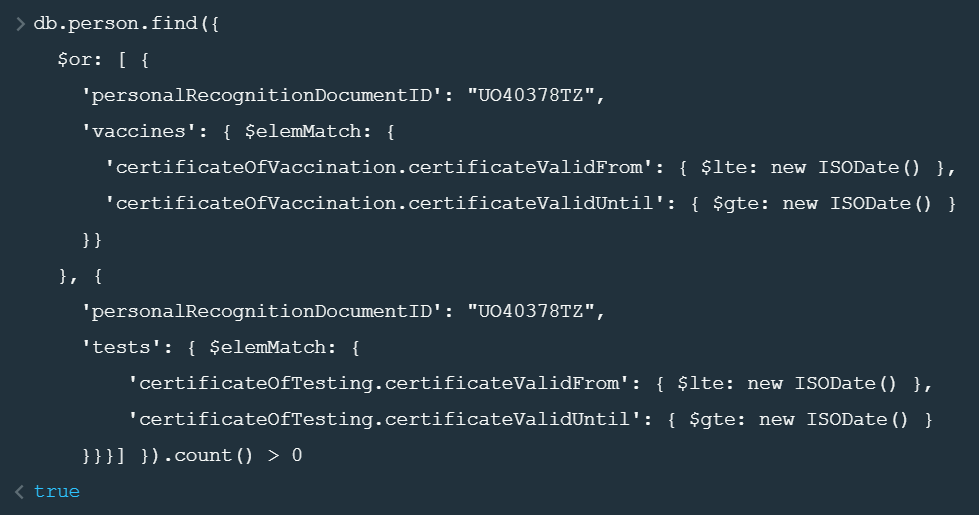
\includegraphics[width=\textwidth, frame]{Query1.PNG}
    \caption{Result of Query 1}
\end{center}
\end{figure}

\newpage 

\item \textbf{Get where, when a person did the vaccine, and who was the nurse/doctor who did it.}
\begin{lstlisting}
db.person.aggregate( 
    {$unwind: "$vaccines"},
    {$addFields: {"hubID": {"$toObjectId": "$vaccines.hubID"}}},
    { $lookup: {
        from: 'healthcareService',
        localField:'hubID',
        foreignField: 'vaccineHubs._id',
        as: 'hub'} }, 
    { $lookup: {
        from: 'person',
        localField:'vaccines.healthWorkerPersonalID.$id',
        foreignField:'_id',
        as: 'worker'} }, 
    { $project: {
        "date":"$vaccines.date",
        "place": {
        "city":"$hub.city",
        "address":"$hub.address",
        "region":"$hub.region",
        "state":"$hub.state"
        },
        "worker":"$worker.personalInformation"
}})
\end{lstlisting}

\begin{figure}[H]
\begin{center}
    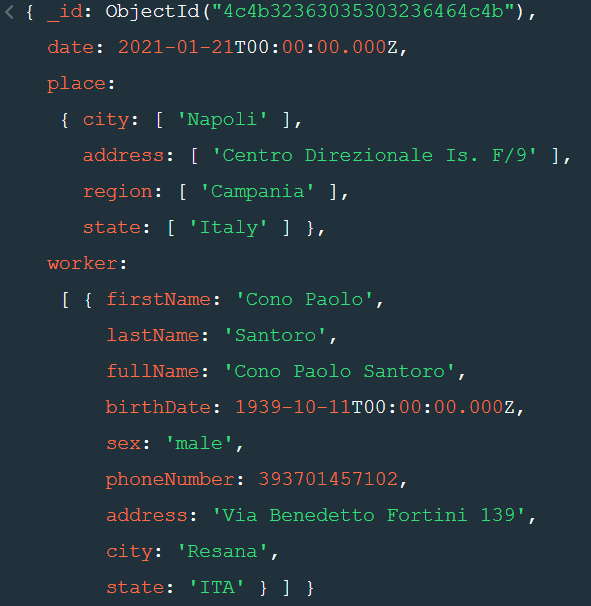
\includegraphics[width=32em]{Query2.PNG}
    \caption{Result of Query 2}
\end{center}
\end{figure}

\newpage 

\item \textbf{Retrieve the emergency contact of a person.}
\begin{lstlisting}
db.person.find(
    {'personalRecognitionDocumentID': 'LK2605026F'},
    {'emergencyContact.phoneNumber':1})
\end{lstlisting}

\begin{figure}[H]
\begin{center}
    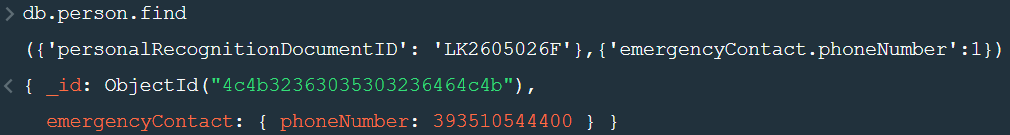
\includegraphics[width=\textwidth]{Query3.PNG}
    \caption{Result of Query 3}
\end{center}
\end{figure}

\item \textbf{Count the number of samples a person has taken.}
\begin{lstlisting}
db.person.aggregate([
    {"$match":{'personalRecognitionDocumentID':"LK2605026F"}},
    {$project:{count:{$size:"$tests"}}}])
\end{lstlisting}

\begin{figure}[H]
\begin{center}
    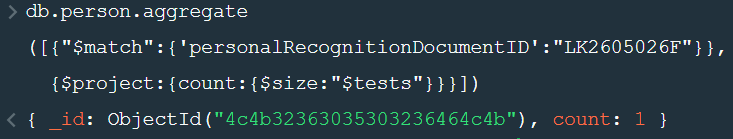
\includegraphics[width=\textwidth]{Query4.PNG}
    \caption{Result of Query 4}
\end{center}
\end{figure}

\item \textbf{Retrieve the amount of people Vaccinated per date}
\begin{lstlisting}
db.person.aggregate([
    {$unwind:"$vaccines"},
    {"$group":{_id:"$vaccines.date",count:{"$sum":1}}}])
\end{lstlisting}

\begin{figure}[H]
\begin{center}
    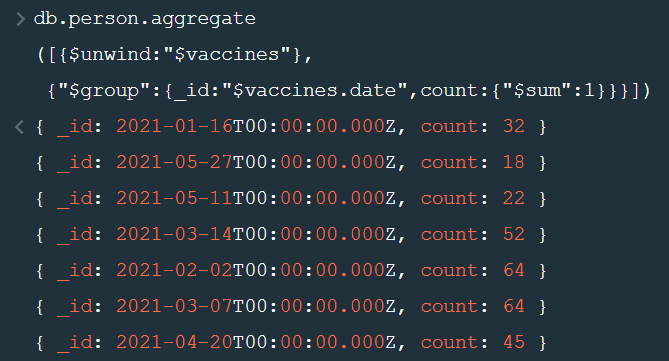
\includegraphics[width=45em]{Query5.PNG}
    \caption{Result of Query 5}
\end{center}
\end{figure}

\item \textbf{Retrieve the top 5 dates per amount of tested people}
\begin{lstlisting}
db.person.aggregate([
    {$unwind:"$tests"},
    {"$group":{_id:"$tests.date",count:{"$sum":1}}},
    {$sort:{"count":-1}},{$limit:5}])
\end{lstlisting}

\begin{figure}[H]
\begin{center}
    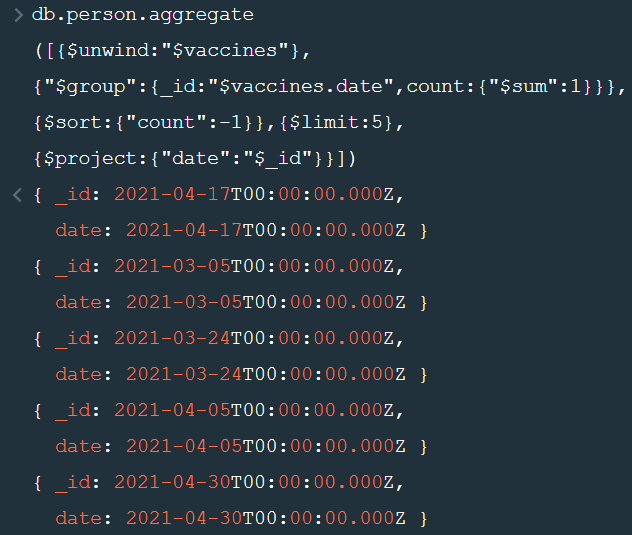
\includegraphics[width=\textwidth]{Query6.PNG}
    \caption{Result of Query 6}
\end{center}
\end{figure}

\newpage 

\item \textbf{Compute the average number of persons tested per Health Service and return the top 5 Health Service per  average persons tested.}
\begin{lstlisting}
db.person.aggregate([
    {$unwind:"$tests"},
    {$lookup: {
        from: 'healthcareService',
        localField: 'tests.healthcareServiceID.$id',
        foreignField: '_id',
        as: 'healthcareServices'
    }},
    {$group: {
        _id:"$healthcareServices.name",
        count:{$sum:1}}},
    {$sort:{"count":-1}},
    {$limit:5}])
\end{lstlisting}
\end{itemize}

\begin{figure}[H]
\begin{center}
    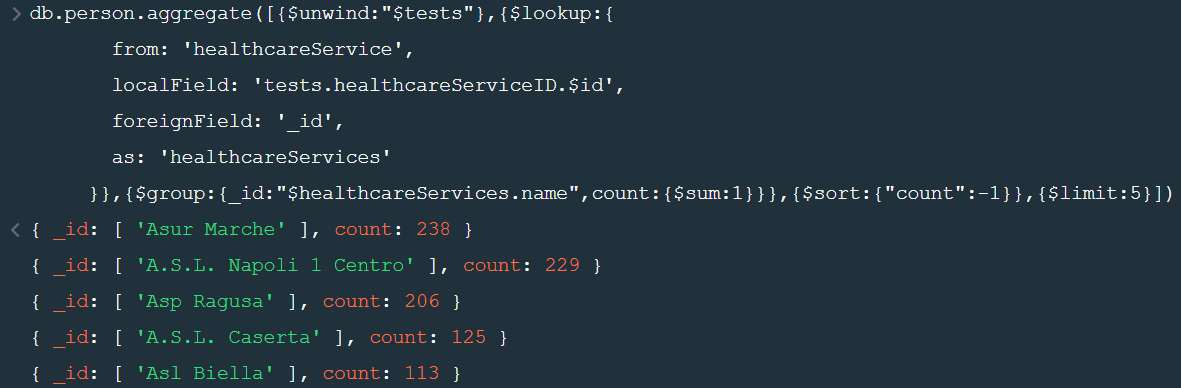
\includegraphics[width=\textwidth]{Query7.PNG}
    \caption{Result of Query 7}
\end{center}
\end{figure}

\newpage 

\subsection{Commands}

The following subsection presents some useful commands, with the aim of showing database’s utility.

\begin{itemize}
    \item \textbf{A person has taken the vaccine:} add it.
    
    \begin{lstlisting}

     db.person.update(
    	{ personalRecognitionDocumentID:"LK2605026F" },
    	{ $push: { vaccines: {
            date: new ISODate("2021-12-11"),
            healthServiceID:{$ref:"healthcareService",
            $id:" 53554d32353953554d323539", 
            $db:"SMBUD"},
            hubID:"414948313335414948313335",
            lotID:{ 
            $ref:"vaccineLot",
            $id:"492876f0ca87930680eb7747", 
            $db:"SMBUD"},
            healthWorkerPersonalID:{
            $ref:"person",
            $id:ObjectId("4c4b32363035303236464c4b"), $db:"SMBUD"},
            certificateOfVaccination: {
                QRCode:"iVBORw0KGgoAAAANSUhEUgAABJIAAASSAQAAA...",
                diseaseOrAgentTargeted:840539006,
                vaccineOrProphylaxis:1119349007,
                vaccineProduct:"EU/1/20/1507",
                uniqueCertificateIdentifier:"01IT5UTPPVIJ713AJCY2...",
                doseNumber:2,
                totalSeriesOfDoses:2,
                countryOfVaccination:"IT",
                marketingAuthorizationHolder:"ORG-100031184",
                certificateIssuer:"Italian Ministry of Health",
                certificateValidFrom: new ISODate("2021-12-20"),
                certificateValidUntil:new ISODate("2022-09-20"),
                schemaVersion:"1.0.0"
            }
        }}}
    )
        \end{lstlisting}
        
        \item \textbf{Delete the first covid test a person has taken.}
         \begin{lstlisting}
        db.person.update( 
            { personalRecognitionDocumentID:"LK2605026F" }, 
            { $unset: {'tests.0':1} } )
        db.person.update( 
            { personalRecognitionDocumentID:"LK2605026F" }, 
            { $pull: { tests:null } } )
        \end{lstlisting}
        
        \item \textbf{Update the emergency phone number of a person.}
         \begin{lstlisting}
        db.person.update(
            { personalRecognitionDocumentID:"LK2605026F" },
            { $set: { 'emergencyContact.phoneNumber':"393510544400" } }
        )
        \end{lstlisting}
 \end{itemize}

\appendix
\section{Delivery content}
Apart from this report, the delivery folder also contains the following files:
\begin{itemize}
    \item \textbf{Python scripts} to create CSVs and database. The Python project is mainly composed by 4 files
    \begin{itemize}
        \item \textbf{csvmanipulation.py}: it contains various utility functions to generate random data\&manipulate CSV files.
        \item \textbf{main.py}: it contains a class to handle database connection and collections/documents creation through various functions.
        \item \textbf{qrcodeutils.py}: it contains various utility functions to encode text, generate, read and recognize qr codes, decode strings related to certificates. 
        \item \textbf{utils.py}: it contains various utility function to generate pseudo random data, such as phone numbers and document ids.
        
    \end{itemize}
    \item \textbf{Folders} containing the various versions of CSVs files, to keep track of the subsequent modifications (these are located inside the Python project folder, inside the \textbf{datasets} folder)
    \item \textbf{Database dump} file.
    \item \textbf{Text file} with queries\&commands.
    
\end{itemize}


%===========================================================
%===========================================================

\bibliographystyle{ieeetr}
\bibliography{refs}


\end{document}